\documentclass{article}

\title{Inverses in Higher Categories}
\author{Alex Rice}

\usepackage{verbatim}
\usepackage[nomarginpar]{geometry}
\usepackage{amsmath}
\usepackage{amssymb}
\usepackage{amsfonts}
\usepackage{mathtools}
\usepackage{amsthm}
\usepackage{cleveref}
\usepackage{tikz}
\usepackage{listings}

\lstset{basicstyle=\ttfamily,
mathescape=true}

\usetikzlibrary{positioning}

\usepackage[
backend=biber,
style=numeric,
citestyle=numeric,
maxbibnames=99,
isbn=false,
doi=false,
eprint=false,
block=ragged
]{biblatex}

\addbibresource{../citations/citations.bib}

\DefineBibliographyStrings{english}{%
  bibliography = {References},
}

\newtheorem{theorem}{Theorem}
\newtheorem{prop}{Proposition}
\newtheorem{cor}{Corollary}
\newtheorem{lemma}{Lemma}
\theoremstyle{definition}
\newtheorem{definition}{Definition}
\newtheorem{remark}{Remark}
\newtheoremstyle{examplestyle}% name
{20pt}% Space above
{20pt}% Space below
{\rmfamily}% Body font
{}%Indent amount (empty = no indent, \parindent = para indent)
{\bfseries}% Thm head font
{.}% Punctuation after thm head
{ }% Space after thm head: " " = normal interword space;
% \newline = linebreak
{}% Thm head spec
\theoremstyle{examplestyle}
\newtheorem{example}{Example}

\DeclareMathOperator{\id}{id}

\newcommand{\linv}[1]{{}^\star\!#1}
\newcommand{\rinv}[1]{#1^\star}
\newcommand{\inv}[1]{#1^{-1}}


\begin{document}
\maketitle

\section{Introduction}\label{sec:intro}

In the study of higher category theory, the notion of invertibility is central. It is common within higher category theory to not specify that two objects are equal, or that two sides of an equation are equal, but rather specify that there is a higher level equivalence between these two objects. It is usual to say that two objects are equivalent exactly when there is an invertible function between them.

This idea can be seen even in the simplest examples of higher categories. Consider the definition of a monoidal category. It is our intention that given objects \(A\), \(B\) and \(C\) that \(A \otimes (B \otimes C)\) and \((A \otimes B) \otimes C\) represent the same object. However it is often the case that requiring equality between these objects (as in a strict monoidal category) is too restrictive and so the usual definition states that there is a natural isomorphism between them.

This is our first example of invertibility. An isomorphism between \(A\) and \(B\) is a morphism \(f : A \to B\) such that there exists a morphisms \(g : B \to A\) with \(f \circ g = \id_B\) and \(g \circ f = \id_A\). This notion of isomorphism works well throughout standard category theory and even in monoidal categories.

However if generalised higher categories are considered, it can be seen that the problem has just been pushed one level up. We have specified that \(g \circ f\) and \(\id_A\) should be equal, yet have already stated that equality is not the best notion of two objects in a higher category. Ideally we want a collection of data that specifies that \(f\) has an inverse \(g\), and that there is a higher morphisms \(\alpha : g \circ f \to \id_A\) and an inverse \(\beta : \id_A \to g \circ f\), and that there exists a morphism \(\alpha \circ \beta \to \id_{\id_A \to g \circ f}\) and continuing in this fashion. Unfortunately this generates a very unwieldy set of data that is difficult to describe.

A natural way we can talk about data structures like this is through coinduction. The definition of equivalence above can be written nicely by saying that \(f : A \to B\) is an equivalence if there exists a \(g : B \to A\) and equivalences \(f \circ g \to \id_B\) and \(g \circ f \to \id_A\). This is a neat method of defining an equivalence, but also has the advantage of opening up more proof techniques to us. In particular, it allows us to structure proofs coinductively.

Given this coinductive machinery, the definition of equivalence above seems very natural. If we start with our definition of isomorphism, then realise that the equalities introduced should themselves be weakened to equivalences, we end up with the proposed definition. However this is not only way we could have defined invertibility. In type theory and in particular in HoTT~\cite{hottbook}, there are 3 notions of invertibility defined:

\begin{itemize}
\item A quasi-inverse, which is similar to the notion of isomorphism presented already;
\item A bi-inverse, where instead of specifying an inverse to the function \(f\), we instead present separate left and right inverses;
\item A half-adjoint inverse, defined to be the same as the quasi-inverse but with an extra coherence condition.
\end{itemize}

There are certain properties about these invertibility conditions that are important in type theory. Firstly, all 3 definitions are equivalent, in that a function \(f\) has one of these 3 types of inverses, then it also has the other 2. Secondly, definitions 2 and 3 form contractible types. In essence, this means that there is only one way in which they hold up to propositional equality.

Although it seems that these 3 are not applicable to generalised higher categories due to the use of equality in their definitions, they can nonetheless be modified into coinductive definitions suitable for such a category. This paper will present those definitions and to attempt to show that they are all equivalent. Further we will try to present an analogue to contractibility which is suitable for higher categories and investigate whether these data types are contractible.

\section{Background}\label{sec:background}

\subsection{Coinduction}\label{sec:coinduction}

Throughout the paper, we want to use coinductive data structures and many functions will be generated by corecursion, and many proofs made using coinduction. Like inductive data structures, coinductive data structures are able to reference themselves in their definition.

Categorically, coinduction forms the categorical dual of induction. Whereas inductive data structures can be thought of as initial algebras, coinductive data structures may be thought of as terminal coalgebras. To see the differences clearly between these two constructions and how they relate, it will be helpful to go through an example. Since a lot of the language used throughout this paper is type-theoretic, induction and coinduction will be explained in the same way. This has the added benefit of being very precise.

When a type is introduced in type theory, there are four parts of its definition: Type formation, Term formation, a recursion principle, and an induction principle. These will be demonstrated with the example of lists.
\begin{itemize}
\item Type formation tells us how to build the type. For lists, given a type \(A\), the type \(\mathsf{List}(A)\) can be formed.
\item Term formation tells us how terms of the type can be constructed. \(\mathsf{List}(A)\) has multiple constructors. We have \(\mathsf{nil} : \mathsf{List}(A)\), which is a constructor with no arguments and \(\mathsf{cons} : A \to \mathsf{List}(A) \to \mathsf{List}(A)\), which takes two.
\item Recursion lets us form functions out of an inductive type. For lists this says that to form a function \(f : \mathsf{List}(A) \to B\), it suffices to define \(f(\mathsf{nil}) : B\) and define \(f(\mathsf{cons}(a)(xs))\) given the value of \(f(xs)\).
\item Induction is a generalisation of recursion and allows us to define functions \(f : \Pi_{xs : \mathsf{List}(A)} P(xs)\) where \(P\) is a type family of type \(\mathsf{List}(A) \to \mathcal{U}\).
\end{itemize}

A further thing to note is that we will require the use of a slight generalisation of this known as inductive type families. These are described in Section~5.7 of \citetitle{hottbook}~\cite{hottbook}. These allow our inductive types to be parameterised. A good example of this is the vector type, which is a list of specified length. Here our type formation rule says that given a type \(A\) we can get a type \(\mathsf{Vec}(A) : \mathbb{N} \to \mathcal{U}\). Further the term formation rules become \(\mathsf{nil} : \mathsf{Vec}(A)(0)\) and \(\mathsf{cons} : \Pi_{n : \mathbb{N}} A \to \mathsf{Vec}(A)(n) \to \mathsf{Vec}(A)(\mathsf{succ}(n))\). Notice that unlike with lists, which also took a parameter, vectors can not be defined by considering each element of the parameter separately. The recursion and induction rules also need to modified slightly.

Now it will be seen how this differs for coinductive types. For this we will use one of the most common coinductive types, the stream.

\begin{itemize}
\item Type formation remains the same as before. Given any type \(A\) we can form \(\mathsf{Stream}(A)\).
\item Instead of specifying how to form terms, we specify how to deconstruct terms. Streams have two deconstructors: \(\mathsf{head} : \mathsf{Stream}(A) \to A\) and \(\mathsf{tail} : \mathsf{Stream}(A) \to \mathsf{Stream}(A)\).
\item Instead of recursion, we have corecursion, which specifies how to build functions \(f : B \to Stream(A)\). Whereas in recursion, we specified the behaviour of the function on each constructor, in corecursion we specify how to deconstruct the value returned. Therefore it suffices to provide \(\mathsf{head}(f(b)) : A\) and to provide \(\mathsf{tail}(f(b)) : \mathsf{Stream}(A)\), where we can use the function \(f\) when defining \(\mathsf{tail}(f(b))\).
\item Coinduction does not work quite the same as induction, as flipping the arrow no longer works due to the dependency in the type. Instead, if we are trying to prove a predicate \(P : \mathsf{Stream}(A) \to \mathcal{U}\), we can define the predicate coinductively, and then provide a witness to it by corecursion. Coinductive type families will likely be needed to define the predicate.
\end{itemize}

As an example of coinduction, suppose we wanted to prove every element of a stream was even. First we construct the predicate \(P : \mathsf{Stream}(\mathbb{N}) \to \mathcal{U}\) as having deconstructors \(\mathsf{headProof}(xs) = \mathsf{is-even}(\mathsf{head}(xs))\) and \(\mathsf{tailProof}(xs) = P(\mathsf{tail}(xs))\). This could then be proved by corecursion.

\subsection{\(\omega\)-categories}\label{sec:categories}

In this paper we want to talk about different structures on \(\omega\)-categories, however there are many different definitions of \(\omega\)-categories, a lot of which are very in depth and complicated. Therefore, similar in style to a paper by \citeauthor{Cheng2007}~\cite{Cheng2007}, we give a set of conditions that we expect to hold in any reasonable definition of a weak infinity category. We then prove results only using these conditions, and reason that given a precise definition of an infinity category, if one could show that these conditions hold, then our results should follow for free.

\begin{definition}
  The globe category \(\mathbb{G}\) is the category where the objects are the natural numbers and morphisms are generated by
  \begin{align*}
    &\sigma_n : n \to n+1\\
    &\tau_n : n \to n+1
  \end{align*}
  subject to the conditions
  \begin{align*}
    \sigma \circ \sigma &= \tau \circ \sigma\\
    \sigma \circ \tau &= \tau \circ \tau
  \end{align*}
\end{definition}

\begin{definition}
  A globular set \(G\) is a presheaf of \(\mathbb{G}\). We refer to \(G(n)\) as the set of \(n\)-cells and for two \(n\)-cells \(x\) and \(y\) we write \(f: x \to y\) to mean that \(f\) is an \((n+1)\)-cell and
  \begin{align*}
    G(\sigma_n)(f) &= x\\
    G(\tau_n)(f) &= y
  \end{align*}
  where we call \(x\) the source of \(f\) and \(y\) the target of \(f\).
\end{definition}

\begin{definition}
  A globular set with identities and composition is a globular set \(G\) with the following:
  \begin{itemize}
  \item For each \(n\)-cell \(x\), there is an \((n+1)\)-cell, \(\id_x\).
  \item Inductively define composition as follows:
    \begin{itemize}
    \item Given \(n\)-cells \(f: x \to y\) and \(g: y \to z\) there is
      an \(n\)-cell \(g \circ_0 f: x \to z\).
    \item Given \(\alpha: f \to g\) and \(\beta: h \to j\), where the composites \(f \circ_n h\) and \(g \circ_n j\) are well defined, there is a morphism \(\alpha \circ_{n+1} \beta: (f \circ_n h) \to (g \circ_n j)\)
    \end{itemize}
  \end{itemize}
  \(\circ\) will be used to mean \(\circ_0\).
\end{definition}

Once we have a globular set with identities and composition, we have enough to define a notion of equivalence. The most basic notion of invertibility will be given here, as it will be needed to state the remainder of properties that we expect an higher category to obey.

\begin{definition}
  Given a globular set \(G\) with identities and composition, with an \(n > 0\) cell \(f : x \to y\), we say that \(f\) is \emph{invertible} if:
  \begin{itemize}
  \item There exists an \(n\)-cell \(\inv f : y \to x\);
  \item There exists an \((n+1)\)-cell \(f_R: f \circ \inv f \to \id_y\);
  \item There exists an \((n+1)\)-cell \(f_L: \inv f \circ f \to \id_x\).
  \item \(f_R\) is invertible.
  \item \(f_L\) is invertible.
  \end{itemize}
\end{definition}

\begin{remark}
  The previous definition is a coinductive one. Formally, we have defined a coinductive data type, which we could call \(\text{Invertible}(f)\), which references itself (in saying that \(f_R\) and \(f_L\) are themselves invertible), and then have specified that \(f\) is invertible if there is a member of \(\text{Invertible}(f)\). Note that as \(\text{Invertible}\) is dependent on the parameter \(f\), it is in fact a coinductive type family as described in Section~\ref{sec:coinduction}.
\end{remark}

\begin{remark}\label{descendants}
  Notice that in a globular set \(G\) with identities and composition, given two \(n\)-cells \(x\) and \(y\) with the same source and target, we can define a new globular set \(G\) as follows:
  \begin{itemize}
  \item The \(0\)-cells are the \(n+1\)-cells in \(G\) with source \(x\) and target \(y\);
  \item The \(m\)-cells are the \(n+m+1\)-cells in \(G\) whose source and target lie in the \(m-1\)-cells of the globular set being generated.
  \end{itemize}
  Further it is clear that we can carry over identities and composition to this new globular set.
\end{remark}



\begin{definition}\label{def:higher-cat}
  Consider the standard string diagram diagrammatic calculus for bicategories. We can draw diagrams containing nodes, lines, and areas where areas represent \(0\)-cells, a line between areas representing cells \(x\) and \(y\) represents a \(1\)-cell between \(x\) and \(y\), and node between lines represent \(2\)-cells between the cells those lines represent. These diagrams still represent well formed morphisms in an globular set with identities and composition. In a bicategory we have the theorem that given a planar isotopy of string diagrams, the source and target morphisms are equal.

  In this higher categorical setting we can instead require that given a well typed string diagram, and an isotopy of this diagram, there is a \(3\)-cell from source of the isotopy to the target. We require that this cell is invertible. We say that a globular set \emph{respects the graphical calculus} if it has this property.

  We define a \emph{higher category} to be a globular set with identities and composition such that given any globular set generated as in \cref{descendants} respects the graphical calculus. Further we assume the existence of the following morphisms.
  \begin{itemize}
  \item For \(n>0\) and each \(n\)-cell \(f: x \to y\), there are \(n+1\)-cells, known as unitors, \(\lambda_f: \id_y \circ f \to f\).
  \item Given \(f,g,h,j\), \(n>1\)-cells with suitable composition defined, we have an associator \(a_{f,g,h,j} : (f \circ g) \circ (h \circ j) \to f \circ ((g \circ h) \circ j)\).
  \item For compatible morphisms \(f,g,h,j\), we have an interchanger \(i_{f,g,h,j}(f \circ_n g) \circ (h \circ_n j) \to (f \circ h) \circ_n (g \circ j)\).
  \item For suitable \(f,g\) and \(n > 1\), there is a cell \(\id_f \circ_{n+1} \id_g \to \id_{f \circ_n g}\)
  \end{itemize}
  All these further morphisms must be invertible.
\end{definition}.

To end this section we give a small lemma, which demonstrates the use of these higher categories and will also be invaluable later.

\begin{lemma}\label{lem:identity}
  Any identity morphism is invertible.
\end{lemma}

\begin{proof}
  Let \(x\) be any cell. Take \(\inv {\id_x} = \id_x\) and \({(\id_x)}_R = {(\id_x)}_L = \lambda_{id_x}\). By assumption, \(\lambda_{id_x}\) is invertible. Hence \(\id_x\) is invertible.
\end{proof}

\section{Types of Invertibility}\label{sec:invertibility}

In this section we introduce 2 more types of invertibility. Some theorems are proved that help us to work with them and finally all 3 types of invertibility are shown to imply each other.

\subsection{Bi-invertibility}\label{sec:bi-invertibility}

Normally, throughout mathematics, when saying a map is invertible we specify a single inverse, and show that this cancels the function when composed on the left and the right. Instead we can consider a function either having a left inverse or a right inverse, meaning the inverse only cancels the function on when composed on the left (or right respectively). It usually does not make sense to consider functions which have both a separate left and right inverse as in most scenarios it can be proved that these are equal and any computations will be simplified by treating them as the same.

However, the concept of bi-invertibility (having both a left and right inverse), plays a role in type theory. It can be shown (perhaps not surprisingly) that a morphism being bi-invertible implies that it is invertible in the usual sense. Perhaps more surprisingly, the data for being bi-invertible is in some ways simpler than the data for being invertible, in that it can be shown that any two ways of showing a function is bi-invertible turn out to be equivalent.

First, we must define what we mean for a morphism in a higher category to be bi-invertible, as a generalisation of the idea in type theory.

\begin{definition}
  Given a globular set \(G\) with identities and composition, with an \(n > 0\) cell \(f : x \to y\), we coinductively say that \(f\) is \emph{bi-invertible} if:
  \begin{itemize}
  \item There exists an \(n\)-cell \(\rinv f : y \to x\);
  \item There exists an \(n\)-cell \(\linv f : y \to x\);
  \item There exists an \((n+1)\)-cell \(f_R: f \circ \rinv f \to \id_y\);
  \item There exists an \((n+1)\)-cell \(f_L: \linv f \circ f \to \id_x\).
  \item \(f_R\) is bi-invertible.
  \item \(f_L\) is bi-invertible.
  \end{itemize}
\end{definition}

Next it is shown that invertibility implies bi-invertibility. This is fairly trivial though it will be written out to demonstrate proof by coinduction.

\begin{lemma}
  Let \(G\) be a globular set with identities and composition. Let \(f : x \to y\) be a cell of \(G\) and suppose \(f\) is invertible. Then \(f\) is bi-invertible.
\end{lemma}

\begin{proof}
  This is proven by constructing a corecursive function \(\mathsf{invToBiInv} : \Pi_{f : x \to y} \mathsf{Invertible}(f) \to \mathsf{BiInvertible}(f)\). Given \(I = (f',f_R^i,f_L^i,f_R{}I, f_L{}I) : \mathsf{Invertible}(f)\) we can construct \(\mathsf{invToBiInv}(f)(I)\) by:
  \begin{itemize}
  \item \(\rinv f = f'\);
  \item \(\linv f = f'\);
  \item \(f_R = f_R^i\);
  \item \(f_L = f_L^i\);
  \item \(f_R\) is bi-invertible corecursively by \(\mathsf{invToBiInv}(f_R)(f_R{}I)\);
  \item \(f_L\) is bi-invertible corecursively by \(\mathsf{invToBiInv}(f_L)(f_L{}I)\).
  \end{itemize}
\end{proof}

\noindent Now, one of the most important and complex theorems of the paper is proved.

\begin{theorem}[Composition of Bi-invertible Morphisms]
  For any \(n \in \mathbb{N}\) and bi-invertible cells \(f,g\), \(f \circ_n g\) is bi-invertible if it is well defined.
\end{theorem}
\begin{proof}
  The proof has a nested coinductive structure. We wish to describe a procedure taking the data that a pair of compatible cells are bi-invertible cells to a proof of bi-invertibility of their composite. This is done by coinductively assuming that this can be done for all \(k\)-cells where \(k>k'\), then showing that such a procedure exists that works for \(k'\)-cells.

  Now take a compatible composition. Split into cases on \(n\):
  \begin{itemize}
  \item \(n = 0\): We need to show \(g \circ f\) is bi-invertible. Let:
    \begin{itemize}
      \item \(\rinv {(g \circ f)} = \rinv f \circ \rinv g\)
      \item \(\linv {(g \circ f)} = \linv f \circ \linv g\)
      \item \({(g \circ f)}_R : g \circ f \circ \rinv f \circ \rinv g\) is the morphism given by the diagram
        \begin{center}
          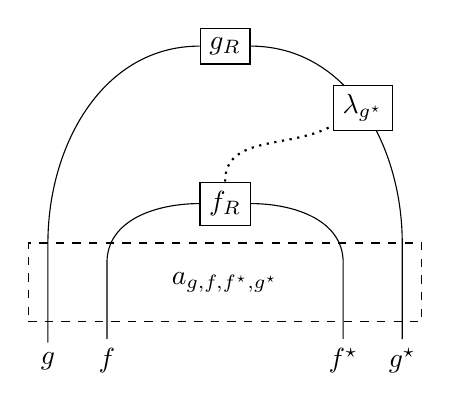
\begin{tikzpicture}
            \node[draw] (GR) {\(g_R\)};
            \node[on grid, below=2 of GR, draw] (FR) {\(f_R\)};
            \node[on grid, below=1 of FR, draw, dashed, minimum width=5cm, minimum height = 1cm] (A) {\(a_{g,f,\rinv f,\rinv g}\)};
            \node[on grid, below left=2cm and 2.25cm of FR] (Base1) {\(g\)};
            \node[on grid, right=0.75cm of Base1] (Base2) {\(f\)};
            \node[on grid, right=3cm of Base2] (Base3) {\(\rinv f\)};
            \node[on grid, right=0.75cm of Base3] (Base4) {\(\rinv g\)};
            \draw (Base1) to ++(0,1.5cm) to [out=90,in=180]  (GR);
            \draw (Base4) to ++(0,1.5cm) to [out=90,in=0] node[fill=white,pos=0.5,draw](L){\(\lambda_{\rinv g}\)} (GR);
            \draw [dotted, thick, out=90,in=-150] (FR) to (L);
            \draw (Base2) to ++(0,1.25cm) to [out=90,in=180] (FR);
            \draw (Base3) to ++(0,1.25cm) to [out=90,in=0] (FR);
          \end{tikzpicture}
        \end{center}
        Here the associator and unitor have been added and a dotted line has been drawn for the identity, even though these would not appear on the standard graphical calculus. This is just to make precise which components of the higher category we are using. Written out in full this morphism is:
        \begin{equation*}
          a_{g,f,\rinv f,\rinv g} \circ_0 (\id_g \circ_1 (f_R \circ_1 \id_{\rinv g})) \circ_0 (\id_g \circ_0 \lambda_{\rinv g}) \circ_0 g_R
        \end{equation*}
      \item \({(g \circ f)}_L\) is the morphism given by the diagram:
        \begin{center}
          \begin{tikzpicture}
            \node[draw] (GL) {\(g_L\)};
            \node[on grid, below=2 of GL, draw] (FL) {\(f_L\)};
            \node[on grid, below=1 of FL, draw, dashed, minimum width=5cm, minimum height = 1cm] {\(a_{\linv g,\linv f, f,g}\)};
            \node[on grid, below left=2cm and 2.25cm of FL] (Base1) {\(\linv g\)};
            \node[on grid, right=0.75cm of Base1] (Base2) {\(\linv f\)};
            \node[on grid, right=3cm of Base2] (Base3) {\(f\)};
            \node[on grid, right=0.75cm of Base3] (Base4) {\(g\)};
            \draw (Base1) to ++(0,1.5cm) to [out=90,in=180] (GL);
            \draw (Base4) to ++(0,1.5cm) to [out=90,in=0] node[fill=white,pos=0.5,draw](L){\(\lambda_{\rinv g}\)} (GL);

            \draw [dotted, thick, out=90,in=-150] (FR) to (L);
            \draw (Base2) to ++(0,1.25cm) to [out=90,in=180] (FL);
            \draw (Base3) to ++(0,1.25cm) to [out=90,in=0] (FL);
          \end{tikzpicture}
        \end{center}
        Similarly this is given by the equation:
        \begin{equation*}
          a_{\linv g, \linv f, f ,g}
        \end{equation*}
      \end{itemize}

      Using that \(f_L\), \(g_L\), \(f_R\),\(g_R\) are bi-invertible as \(f\) and \(g\) are bi-invertible and further using the coinductive hypothesis that bi-invertibility is preserved by both \(\circ_0\) and \(\circ_1\) for \((k'+1)\)-cells, we deduce that both \({(g \circ f)}_R\) and \({(g \circ f)}_L\) are bi-invertible and so \(g \circ f\) is bi-invertible.
    \item \(\alpha \circ_n \beta\) where \(n > 0\), \(\alpha: f \to g\), and \(\beta: h \to j\): Let:
      \begin{itemize}
      \item \(\rinv {(\alpha \circ_n \beta)} = \rinv \alpha \circ_n \rinv \beta\)
      \item \(\linv {(\alpha \circ_n \beta)} = \linv \alpha \circ_n \linv \beta\)
      \item Define \({(\alpha \circ_n \beta)}_R\) as the following composition:
        \begin{equation*}
          (\alpha \circ_n \beta) \circ (\rinv \alpha \circ_n \rinv \beta) \overset {i_{\alpha,\beta,\rinv \alpha, \rinv \beta}} \to (\alpha \circ \rinv \alpha) \circ_n (\beta \circ \rinv \beta) \overset {\alpha _R \circ_{n+1} \beta _R} \to \id_g \circ_n \id_j \to \id_{g \circ_{n-1} j}
        \end{equation*}
      \item Similarly, define \({(\alpha \circ_n \beta)}_L\) as the following composition:
        \begin{equation*}
          (\linv \alpha \circ_n \linv \beta) \circ (\alpha \circ_n \beta) \overset {i_{\linv \alpha, \linv \beta, \alpha, \beta}} \to (\linv \alpha \circ \alpha) \circ_n (\linv \beta \circ \beta) \overset {\alpha _L \circ_{n+1} \beta _L} \to \id_f \circ_n \id_h \to \id_{f \circ_n h}
        \end{equation*}
    \end{itemize}
    Now I claim that both \({(\alpha \circ_n \beta)}_R\) and \({(\alpha \circ_n \beta)}_L\) are both bi-invertible. This is because these are compositions of cells that are bi-invertible and these cells are of a higher order than \(k'\) and so we can apply the coinductive hypothesis. Hence \(\alpha \circ_n \beta\) is bi-invertible.
  \end{itemize}
\end{proof}
A comment should be made on why this is a valid coinductive proof.

\begin{lemma}[Inverses are bi-invertible]
  \label{lem:inverses}
  Let \(f\) be a bi-invertible cell. Then \(\linv f\) and \(\rinv f\) are bi-invertible.
\end{lemma}
\begin{proof}
  We show \(\rinv f\) is bi-invertible and \(\linv f\) will follow similarly. Define the following:
  \begin{itemize}
  \item \(\rinv {(\rinv f)} = f\)
  \item \(\linv {(\rinv f)} = f\)
  \item \((\rinv f)_R: \rinv f \circ f \to \id\) is given by:
    \begin{center}
      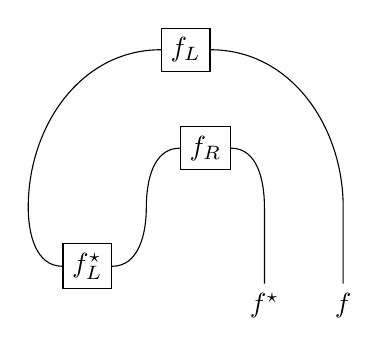
\begin{tikzpicture}
        \node (Finv) {\(\rinv f\)};
        \node [on grid, right=1cm of Finv] (F) {\(f\)};
        \node [on grid, above left=2cm and 0.75cm of Finv, draw] (FR) {\(f_R\)};
        \node [on grid, below left=1.5cm and 1.5cm of FR, draw] (FLInv) {\(\rinv {f_L}\)};
        \node [on grid, above right=2.75cm and 1.25cm of FLInv, draw] (FL) {\(f_L\)};
        \draw (Finv) to ++(0,1.25cm) to[out=90,in=0] (FR);
        \draw (FR) to[out=180,in=90] ++(-0.75cm,-0.75cm) to[out=-90,in=0] (FLInv);
        \draw (FLInv) to[out=180,in=-90] ++(-0.75cm,0.75cm) to[out=90,in=180] (FL);
        \draw (F) to ++(0,1.25cm) to[out=90,in=0] (FL);
      \end{tikzpicture}
    \end{center}
  \item \((\rinv f)_L: f \circ \rinv f \to \id\) is given by \(f_R\)
  \end{itemize}
  We get that \((\rinv f)_R\) is bi-invertible as it is a composite of bi-invertible morphisms (where \(\rinv {f_L}\) is bi-invertible by coinductive hypothesis) and \((\rinv f)_L\) is trivially bi-invertible.
\end{proof}

\begin{definition}
  We define the collection of \emph{half-adjoint invertible} morphisms coinductively as follows: For \(n > 0\), an \(n\)-cell \(f: x \to y\) is \emph{half-adjoint invertible} if:
  \begin{itemize}
  \item There exists an \(n\)-cell \(f' : y \to x\).
  \item There exists an \(n+1\)-cell \(\alpha: f \circ f' \to \id_y\).
  \item There exists an \(n+1\)-cell \(\beta: \id_x \to f' \circ f\).
  \item There exists an \(n+2\)-cell \(\gamma: (\lambda_{f'} \circ (\beta \circ_1 \id_{f'}) \circ (\id_{f'} \circ_1 \alpha) \circ \rho_{f'}) \to \id_{f'}\).
  \item \(\alpha\) is \emph{half-adjoint invertible}.
  \item \(\beta\) is \emph{half-adjoint invertible}.
  \item \(\gamma\) is \emph{half-adjoint invertible}.
  \end{itemize}

  \(\gamma\) can be graphically represented by the following diagram:
  \begin{center}
    \begin{tikzpicture}
      \node (Bottom) {\({f'}\)};
      \node[on grid, above left=1cm and 2.25cm of Bottom, draw] (Cup){\(\beta\)};
      \node[on grid, above right=2cm and 1.5cm of Cup,draw] (Cap){\(\alpha\)};
      \node[on grid, above left=1cm and 2.25cm of Cap] (Top) {\({f'}\)};
      \draw (Bottom) to++(0,2) to[out=90,in=0] (Cap);
      \draw (Cup) to[out=0,in=-90] ++(0.75,1) to[out=90,in=180] (Cap);
      \draw (Cup) to[out=180,in=-90] ++(-0.75,1) to (Top);

      \node[on grid, above right=2cm and 1cm of Bottom, font=\fontsize{20}{24}\selectfont] (Eq) {\(\Rightarrow\)};
      \node[above=0cm of Eq,font=\fontsize{15}{19}\selectfont] (Gamma) {\(\gamma\)};
      \node[on grid, right=2cm of Bottom] (L1) {\({f'}\)};
      \node[on grid, above=4cm of L1] (L2) {\({f'}\)};
      \draw (L1) to (L2);
    \end{tikzpicture}
  \end{center}
\end{definition}

\begin{theorem}
  A \emph{half-adjoint invertible} morphism is bi-invertible.
\end{theorem}
\begin{proof}
  Suppose \(f\) is \emph{half-adjoint invertible}. Then let:
  \begin{itemize}
  \item \(\rinv f = {f'}\)
  \item \(\linv f = {f'}\)
  \item \(f_R = \alpha\)
  \item \(f_L = \rinv \beta\) (using that \(\beta\) is \emph{half-adjoint invertible} and hence bi-invertible)
  \end{itemize}
  Then by coinduction \(f_R = \alpha\) is bi-invertible and \(\beta\) is bi-invertible and so, by \cref{lem:inverses}, \(\rinv \beta\) is also bi-invertible which means \(f\) is too.
\end{proof}

\begin{theorem}
  A bi-invertible morphism is \emph{half-adjoint invertible}.
\end{theorem}
\begin{proof}
  Let \(f\) be bi-invertible. Then let:
  \begin{itemize}
  \item \({f'} = \rinv f\)
  \item \(\alpha = f_R\)
  \item \(\beta\) is given by the following diagram:
    \begin{center}
      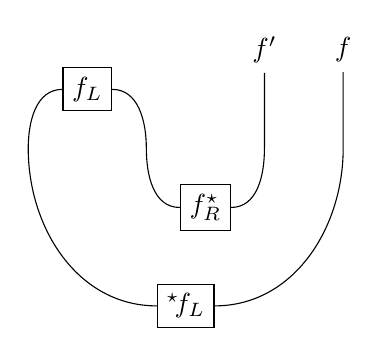
\begin{tikzpicture}
        \node (Finv) {\({f'}\)};
        \node [on grid, right=1cm of Finv] (F) {\(f\)};
        \node [on grid, below left=2cm and 0.75cm of Finv, draw] (FRInv) {\(\rinv {f_R}\)};
        \node [on grid, above left=1.5cm and 1.5cm of FRInv, draw] (FL) {\(f_L\)};
        \node [on grid, below right=2.75cm and 1.25cm of FL, draw] (FLInv) {\(\linv {f_L}\)};
        \draw (Finv) to ++(0,-1.25cm) to[out=-90,in=0] (FRInv);
        \draw (FRInv) to[out=180,in=-90] ++(-0.75cm,0.75cm) to[out=90,in=0] (FL);
        \draw (FL) to[out=180,in=90] ++(-0.75cm,-0.75cm) to[out=-90,in=180] (FLInv);
        \draw (F) to ++(0,-1.25cm) to[out=-90,in=0] (FLInv);
      \end{tikzpicture}
    \end{center}
  \item \(\gamma\) is given by the following diagram:
    \begin{center}
      \begin{tikzpicture}
        \node (G) {\({f'}\)};
        \node [on grid, below right=0.25cm and 1.75cm of G, draw] (FR) {\(f_R\)};
        \node [on grid, below right=5cm and 0.75cm of FR] (G') {\({f'}\)};
        \node [on grid, below left=3cm and 0.75cm of G, draw] (FRInv) {\(\rinv {(f_R)}\)};
        \node [on grid, above left=1.5cm and 1.5cm of FRInv, draw] (FL) {\(f_L\)};
        \node [on grid, below right=2.75cm and 1.25cm of FL, draw] (FLInv) {\(\linv {(f_L)}\)};
        \draw (G) to ++(0,-2.25cm) to[out=-90,in=0] (FRInv);
        \draw (FRInv) to[out=180,in=-90] ++(-0.75cm,0.75cm) to[out=90,in=0] (FL);
        \draw (FL) to[out=180,in=90] ++(-0.75cm,-0.75cm) to[out=-90,in=180] (FLInv);
        \draw (FR) to[out=180,in=90] ++(-0.75cm,-0.75cm) to ++(0,-1.25cm) to[out=-90,in=0] (FLInv);
        \draw (FR) to[out=0,in=90] ++(0.75cm,-0.75cm) to (G');

        \node [on grid, below right=2.75cm and 3.75cm of G,font=\fontsize{20}{24}\selectfont] (A1) {\(\Rightarrow\)};
        \node [on grid, above=0.5cm of A1] (A1Text) {isotopy};

        \node [on grid, right=8cm of G] (G1) {\({f'}\)};
        \node [on grid, below left=2cm and 0.75cm of G1, draw] (FRInv1) {\(\rinv {(f_R)}\)};
        \node [on grid, below=1cm of FRInv1, draw] (FR1) {\(f_R\)};
        \node [on grid, above left=1.5cm and 1.5cm of FRInv1, draw] (FL1) {\(f_L\)};
        \node [on grid, below left=1.5cm and 1.5cm of FR1, draw] (FLInv1) {\(\linv {(f_L)}\)};
        \node [on grid, below right=2cm and 0.75cm of FR1] (G'1) {\({f'}\)};
        \draw (G1) to ++(0,-1.25cm) to[out=-90,in=0] (FRInv1);
        \draw (FRInv1) to[out=180,in=-90] ++(-0.75cm,0.75cm) to[out=90,in=0] (FL1);
        \draw (FL1) to[out=180,in=90] ++(-0.75cm,-0.75cm) to ++(0,-2.5cm) to[out=-90,in=180] (FLInv1);
        \draw (FR1) to[out=180,in=90] ++(-0.75cm,-0.75cm) to[out=-90,in=0] (FLInv1);
        \draw (FR1) to[out=0,in=90] ++(0.75cm,-0.75cm) to (G'1);

        \node [on grid, rotate=-90, below left=1.5cm and 1.5cm of G'1,font=\fontsize{20}{24}\selectfont] (A2) {\(\Rightarrow\)};
        \node [on grid, left=1cm of A2] (A2Text) {\((f_R)_R\)};

        \node [on grid, below=8cm of G1] (G2) {\({f'}\)};
        \node [on grid, below=3.5cm of G2] (G'2) {\({f'}\)};
        \node [on grid, below left=1cm and 2.25cm of G2, draw] (FL2) {\(f_L\)};
        \node [on grid, below=1.5cm of FL2, draw] (FLInv2) {\(\linv {(f_L)}\)};
        \draw (G2) to (G'2);
        \draw (FL2) to[out=0,in=90] ++(0.75cm,-0.75cm) to[out=-90,in=0] (FLInv2);
        \draw (FL2) to[out=180,in=90] ++(-0.75cm,-0.75cm) to[out=-90,in=180] (FLInv2);

        \node [on grid, below left=0.75cm and 2.5cm of FL2,font=\fontsize{20}{24}\selectfont] (A3) {\(\Leftarrow\)};
        \node [on grid, above=0.5cm of A3] (A3Text) {\((f_L)_L\)};

        \node [on grid, below=8cm of G] (G3) {\({f'}\)};
        \node [on grid, below=3.5cm of G3] (G'3) {\({f'}\)};
        \draw (G3) to (G'3);
      \end{tikzpicture}
    \end{center}
    \(\alpha\) is bi-invertible. \(\beta\) is a composite of bi-invertible morphisms and inverses of bi-invertible morphisms so is itself bi-invertible. \(\gamma\) consists of a composition of bi-invertible morphisms and isotopies so is bi-invertible. Therefore all of these are \emph{half-adjoint invertible} by coinduction and so \(f\) is \emph{half-adjoint invertible}.
  \end{itemize}
\end{proof}

\printbibliography
\end{document}